%----------------------------------
\section{Data Analysis}
\label{sec:Data Analysis}
%----------------------------------

\subsection{Method}
\label{subsec:Method}

Both corpora were reduced to the same operational question a moderation queue actually
asks: \emph{should this item be escalated to a human reviewer?} In the Davidson corpus the
positive class is \texttt{hate speech}; in the Wikipedia corpus it is a comment that the
majority of its annotators marked toxic. Text was represented as sublinear TF--IDF over
word unigrams and bigrams, capped at 20,000 features.

Two algorithms were compared: a \textbf{linear support vector
machine}~\cite{cortes1995support}, the standard strong baseline for high-dimensional
sparse text~\cite{joachims1998text}, and a \textbf{feed-forward neural network} with one
64-unit hidden layer, which can represent feature interactions a linear boundary cannot.
Neither was used in previous coursework. Both were implemented with
scikit-learn~\cite{pedregosa2011scikit} and evaluated under stratified five-fold cross
validation. Critically, the vectoriser sits inside the pipeline and is therefore refitted
on each training fold; fitting it once over the whole corpus would leak test-fold
vocabulary into training and inflate every metric reported
below~\cite{pageEvaluating}.

\subsection{Choice of Evaluation Metrics}
\label{subsec:Choice of Evaluation Metrics}

Accuracy is the wrong headline for this case study, and Table~\ref{tab:results} shows why
concretely. On the Davidson corpus the neural network is the \emph{more accurate} model
(94.5\% versus 92.2\%) while being the substantially worse moderation tool: it recovers
13.5\% of hate speech where the SVM recovers 41.1\%. With a 5.77\% positive class, a
model that predicted ``never escalate'' would score 94.2\% accuracy and be
useless~\cite{pageEvaluating}. Four metrics were therefore chosen against the
properties of this problem:

\begin{itemize}
    \item \textbf{Precision and recall} on the positive class, because the two error types
    have different costs and different owners. A false negative leaves harmful content in
    front of users; a false positive removes a legitimate creator's post and generates an
    appeal. Neither is captured by a single accuracy figure.

    \item \textbf{PR-AUC} as the primary threshold-independent score. Both corpora are
    dominated by negatives, the regime in which precision-recall curves are more
    informative than ROC curves, because ROC's false-positive rate is diluted by a very
    large negative denominator and so looks flattering~\cite{davis2006relationship,
    saito2015precision}.

    \item \textbf{ROC-AUC} reported alongside it, since it is insensitive to class
    distribution and therefore the fairer basis for comparing the same model across two
    corpora with different base rates~\cite{pageEvaluating}.

    \item \textbf{Precision@1\%}, the precision over the top 1\% of the ranked stream.
    This is the metric the deployed system is actually judged on: moderator headcount is
    fixed, so what matters is the purity of the queue a reviewer works through, not
    performance at an arbitrary 0.5 threshold.
\end{itemize}

Model comparison uses a paired two-tailed $t$-test over the per-fold differences rather
than a comparison of means, so that fold-to-fold variance is accounted
for~\cite{pageEvaluating}. The test is reported with the caveat that repeated-CV folds
are not fully independent, which makes it liberal~\cite{dietterich1998approximate}.

\begin{table}[h]
\centering
\caption{Five-fold cross-validated performance, averaged across folds. Bold marks the
better of the two models on each row. $p$-values are from paired two-tailed $t$-tests on
per-fold differences. Note that on Dataset~A the neural network is the more accurate model
yet materially the worse moderation tool.}
\label{tab:results}
\begin{tabular}{llcccc}
\toprule
& & \multicolumn{2}{c}{\textbf{Dataset A: Davidson}} & \multicolumn{2}{c}{\textbf{Dataset B: Wikipedia}} \\
\cmidrule(lr){3-4}\cmidrule(lr){5-6}
\textbf{Metric} & & \textbf{Linear SVM} & \textbf{Neural net} & \textbf{Linear SVM} & \textbf{Neural net} \\
\midrule
Accuracy      & & 0.922 & \textbf{0.945} & 0.938 & \textbf{0.957} \\
Precision     & & 0.353 & \textbf{0.619} & 0.640 & \textbf{0.851} \\
Recall        & & \textbf{0.411} & 0.135 & \textbf{0.820} & 0.674 \\
F1            & & \textbf{0.379} & 0.216 & 0.719 & \textbf{0.752} \\
ROC-AUC       & & \textbf{0.829} & 0.801 & 0.959 & 0.960 \\
PR-AUC        & & 0.337 & 0.327 & 0.839 & 0.840 \\
Precision@1\% & & 0.632 & 0.640 & \textbf{1.000} & 0.999 \\
\midrule
\multicolumn{6}{l}{\emph{Paired $t$-test, SVM $-$ neural net:}} \\
$p$ (F1)      & & \multicolumn{2}{c}{0.014$^{*}$} & \multicolumn{2}{c}{$<$0.001$^{*}$} \\
$p$ (PR-AUC)  & & \multicolumn{2}{c}{0.299} & \multicolumn{2}{c}{0.778} \\
$p$ (ROC-AUC) & & \multicolumn{2}{c}{0.012$^{*}$} & \multicolumn{2}{c}{0.651} \\
\bottomrule
\multicolumn{6}{l}{\footnotesize $^{*}$ significant at $\alpha = 0.05$. Base rates: 5.77\% (A), 9.62\% (B).}
\end{tabular}
\end{table}

\subsection{What the Algorithms Reveal}
\label{subsec:What the Algorithms Reveal}

\textbf{The two models rank almost identically; they differ only in where they cut.}
This is the least obvious and most useful result. On both corpora the difference in PR-AUC
is not statistically significant ($p = 0.299$ and $p = 0.778$), and on the Wikipedia
corpus neither is ROC-AUC ($p = 0.651$). Yet precision and recall differ significantly
every time. The two algorithms have learned an equivalent ordering of the data, and every
apparent difference in Table~\ref{tab:results} comes from the operating point rather than
from model capacity --- the SVM was given \texttt{class\_weight="balanced"} and so cuts
aggressively for recall, while the network, trained on the raw imbalance, cuts
conservatively for precision. Figure~\ref{fig:pr curves} shows this directly: the curves
sit on top of one another, and only the points chosen along them differ. For an engineer
this reframes the decision. The choice between these two models is not a modelling
question at all; it is a threshold policy set by how many moderators are rostered.

\textbf{The task is far harder on one corpus than the other.} On Wikipedia both models are
strong: PR-AUC $\approx 0.84$ against a 9.62\% base rate, and precision over the top 1\% of
the ranked stream is effectively perfect (1.000 and 0.999). A reviewer working the head of
that queue would see almost nothing but genuine toxicity. On Davidson both models are
weak: PR-AUC $\approx 0.33$, and precision@1\% of only 0.63. The gap is not a data-volume
artefact --- it is that separating \emph{hate speech} from \emph{merely offensive
language} is intrinsically harder than separating toxic from civil, which is precisely the
problem Davidson et al.\ set out to demonstrate~\cite{davidson2017automated}.

\begin{figure}[h]
    \centering
    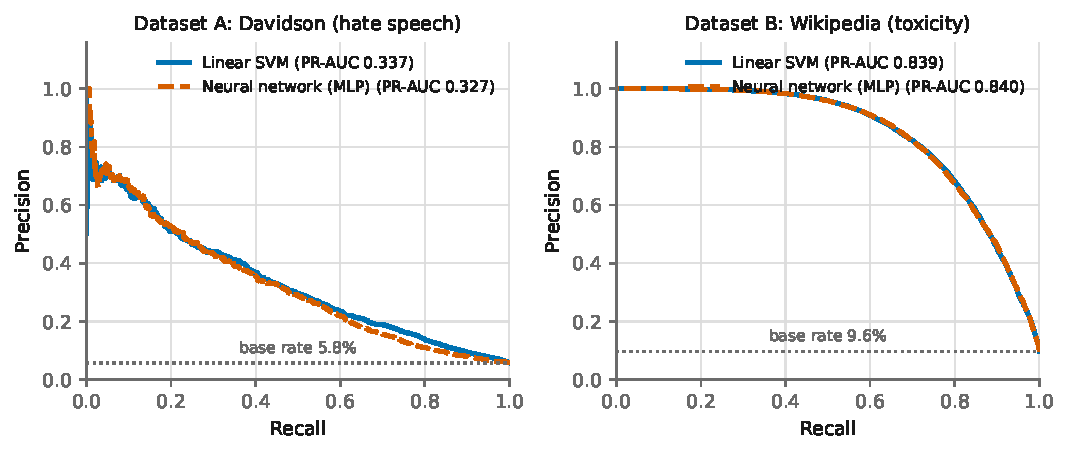
\includegraphics[width=\linewidth]{img/fig_pr_curves.pdf}
    \Description{Two precision-recall panels. On the Davidson corpus both models trace
    nearly identical curves reaching PR-AUC of about 0.33 against a 5.8 percent base rate.
    On the Wikipedia corpus both trace nearly identical curves reaching PR-AUC of about
    0.84 against a 9.6 percent base rate. In both panels the two model curves overlap
    almost exactly.}
    \caption{Precision-recall curves, pooled across folds. The two algorithms are
    near-indistinguishable as \emph{rankers} on both corpora; the significant differences
    in Table~\ref{tab:results} come from threshold placement, not ranking quality.}
    \label{fig:pr curves}
\end{figure}

\begin{figure}[h]
    \centering
    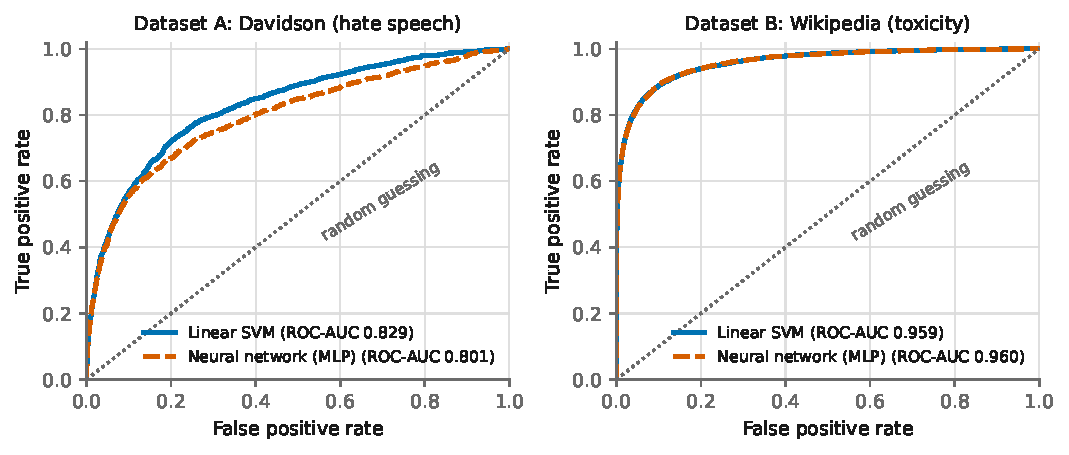
\includegraphics[width=\linewidth]{img/fig_roc_curves.pdf}
    \Description{Two ROC panels. Both models reach ROC-AUC around 0.80 to 0.83 on the
    Davidson corpus and around 0.96 on the Wikipedia corpus, well above the random-guessing
    diagonal.}
    \caption{ROC curves, pooled across folds. ROC-AUC of 0.96 on Dataset~B looks
    excellent, but compare it with the PR-AUC of 0.84 in Figure~\ref{fig:pr curves}: with
    90\% of the corpus negative, the false-positive rate is diluted and ROC flatters the
    models~\cite{davis2006relationship}.}
    \label{fig:roc curves}
\end{figure}

\subsection{Are the Two Sources Complementary or Contradicting?}
\label{subsec:Are the Two Sources Complementary or Contradicting?}

\textbf{Both.} They agree about the models and disagree about the labels, and separating
those two claims is the substantive finding of this analysis.

They are \textbf{complementary about model selection}. Independently, on corpora that
differ by a factor of six in size, by platform, by mean document length and by annotation
protocol, both corpora return the same verdict: the two algorithms rank equivalently and
the SVM achieves it at roughly one-fifth of the training cost. A conclusion that
replicates across two unrelated sources is far stronger than one drawn from either alone.

They are \textbf{directly contradicting about what the label means}, and the contradiction
is severe enough to invalidate any attempt to pool them. Training on Wikipedia and testing
on Davidson, the SVM flags \textbf{73.3\% of the entire stream} against a true base rate of
5.8\%, and precision falls from 0.640 to 0.065 --- ten times worse than the within-corpus
figure. Figure~\ref{fig:transfer} shows why. The Wikipedia-trained SVM flags 82.7\% of
Davidson's hate speech and \emph{82.7\% of its merely offensive language} --- the identical
rate. The model has no discriminative power whatsoever between the two classes, because
the corpus it learned from never encoded a distinction between them. The neural network
behaves the same way, flagging 68.4\% of hate speech and 70.8\% of non-hate offensive
language, if anything inverting the ordering.

\begin{figure}[h]
    \centering
    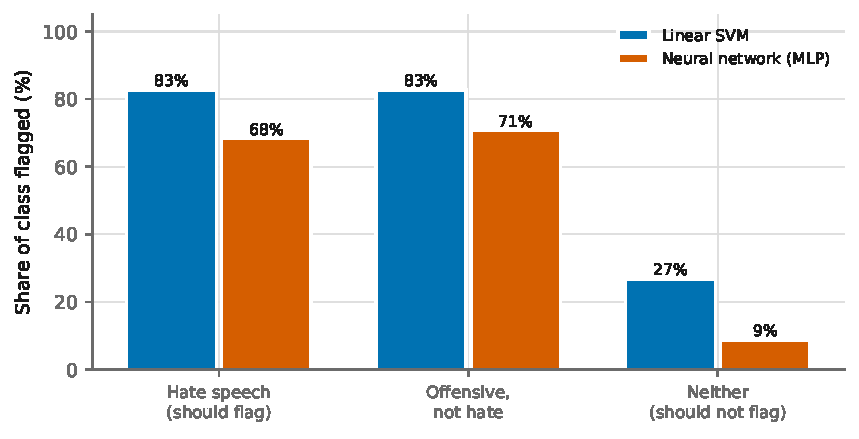
\includegraphics[width=0.72\linewidth]{img/fig_transfer.pdf}
    \Description{A grouped bar chart. A Wikipedia-trained linear SVM flags 83 percent of
    Davidson hate speech and 83 percent of Davidson offensive-but-not-hate content, and 27
    percent of the neither category. The neural network flags 68 percent, 71 percent and 9
    percent respectively. Both models flag the hate and the merely-offensive categories at
    essentially the same rate.}
    \caption{Applying a Wikipedia-trained model to Davidson's data. Both models flag
    genuine hate speech and merely offensive language at effectively the same rate ---
    they cannot tell the two apart, because the Wikipedia label scheme never separated
    them. This is invisible to any single-corpus evaluation.}
    \label{fig:transfer}
\end{figure}

The reverse direction fails differently and just as informatively: a Davidson-trained
neural network flags only 0.8\% of Wikipedia against a 9.6\% base rate, recovering 5.4\% of
genuine toxicity. Trained on a narrow, lexicon-seeded definition, it does not recognise
most of what Wikipedia's annotators consider harmful.

\textbf{Do all data sources give insights? Not equally.} Wikipedia supports a deployable
triage model. Davidson does not --- but its value is diagnostic rather than predictive: it
is the only one of the two that can expose the over-flagging failure at all, precisely
because it preserves the distinction the other corpus collapses. Discarding it as the
``worse'' dataset on PR-AUC would have discarded the finding.

\subsection{Limitations and Implications for Practice}
\label{subsec:Limitations and Implications for Practice}

Three limitations bound these conclusions. Both corpora are English-only and text-only,
whereas the advertised role concerns short-form video across many languages. Majority-vote
aggregation discards annotator disagreement, and disagreement is signal --- an item ten
annotators split evenly on is a different object from one they unanimously cleared. And
the paired $t$-test over five overlapping folds is liberal, so the significant results
above should be read as indicative rather than conclusive~\cite{dietterich1998approximate}.

A further concern is one the metrics here cannot see. Published work shows that classifiers
trained on corpora of this kind systematically over-flag African-American
English~\cite{sap2019risk, blodgett2016demographic}, and the aggregate PR-AUC that looks
healthy on Dataset~B can conceal a much worse error rate for a specific community. The
Wikipedia corpus ships annotator demographics for exactly this reason. Before deployment,
the evaluation in Table~\ref{tab:results} would need to be disaggregated by dialect and
speaker group, not merely repeated at higher precision.

The practical recommendation follows from the first result. Ship the linear SVM: it ranks
as well as the neural network on every threshold-independent measure, trains in roughly a
fifth of the time, and its coefficients can be inspected when a creator appeals a removal.
Then treat the decision threshold as an operational control tied to review capacity rather
than a fixed model property. Most importantly, never validate such a model on a single
labelled source. A system reporting 0.96 ROC-AUC in-corpus flagged three-quarters of a
different platform's traffic, and no amount of cross validation \emph{within} one dataset
would have revealed it~\cite{vidgen2020directions}.
